

% \usepackage{graphicx}% Include figure files
% \usepackage{dcolumn}% Align table columns on decimal point
% \usepackage{bm}% bold math
% %\usepackage[mathlines]{lineno}% Enable numbering of text and display math
% %\linenumbers\relax % Commence numbering lines

% \usepackage[utf8]{inputenc}
% \usepackage[T1]{fontenc}
% \usepackage{mathptmx}
% \usepackage{etoolbox}
% \usepackage{booktabs}
% \usepackage{url}
% \usepackage{hyperref}
% \usepackage{color,graphicx}% color
% \usepackage[dvipsnames]{xcolor}

% \definecolor{grey}{rgb}{0.7,0.7,0.7}

% \definecolor{cNeutralGray}{RGB}{99,101,105}
% \definecolor{cGreenCurrent}{rgb}{0.4660,0.6740,0.1880}
% \definecolor{cEverGreen}{rgb}{0,0.5,0}
% \definecolor{cCyanCurrent}{rgb}{0.3010, 0.7450, 0.9330}
% \definecolor{cBlueSecondary}{RGB}{0, 75, 135}
% \definecolor{cViolet}{RGB}{204, 0, 204}
% \definecolor{cYellow}{RGB}{255, 255, 51}
% \definecolor{cOrangeUtility}{RGB}{242, 160, 0}
% \definecolor{cRedUtility}{RGB}{183, 49, 44}

% \definecolor{cBlueBrand}{RGB}{47, 126, 178}
% \definecolor{cVioletCurrent}{rgb}{0.4940, 0.1840, 0.5560}
% \definecolor{cBlack}{rgb}{0, 0, 0}
% \definecolor{cYellowCurrent}{rgb}{0.9290, 0.6940, 0.1250}


% % \newcommand{\rev}[1]{{\color{red}#1}}
% \newcommand{\rev}[1]{#1}
% \newcommand{\highlight}[1]{{\color{green}[#1]}}
% \newcommand{\revd}[1]{{\color{blue}\sout{#1}}}
% \newcommand{\marco}[1]{\textbf{{\color{cOrangeUtility} [#1] }}}

% %% Apr 2021: AIP requests that the corresponding 
% %% email to be moved after the affiliations
% \makeatletter
% \def\@email#1#2{%
%  \endgroup
%  \patchcmd{\titleblock@produce}
%   {\frontmatter@RRAPformat}
%   {\frontmatter@RRAPformat{\produce@RRAP{*#1\href{mailto:#2}{#2}}}\frontmatter@RRAPformat}
%   {}{}
% }%
% \makeatother



% \begin{document}

% \preprint{AIP/123-QED}

% \title[Skin-friction contributions in adverse-pressure-gradient turbulent boundary layers]{A new perspective on skin-friction contributions in\\adverse-pressure-gradient turbulent boundary layers}
% % Force line breaks with \\
% \author{M. Atzori}
%  \email{marco.atzori@jku.at}
% \affiliation{ 
% Department of Particulate Flow Modelling, Johannes Kepler University, 4040 Linz, Austria %\\This line break forced with \textbackslash\textbackslash
% }%
% \author{F. Mallor}%
% \author{R. Pozuelo}
% \affiliation{ 
%  SimEx/FLOW, Engineering Mechanics, KTH Royal Institute of Technology, 10044 Stockholm, Sweden %\\This line break forced with \textbackslash\textbackslash
% }%

% \author{A. Stroh}
% \author{D. Gatti}
%  %\homepage{http://www.Second.institution.edu/~Charlie.Author.}
% \affiliation{%
% Institute of Fluid Mechanics (ISTM), Karlsruhe Institute of Technology, 76131 Karlsruhe, Germany%\\This line break forced% with \\
% }%

% \author{K. Fukagata}
% \affiliation{ 
% Department of Mechanical Engineering, Keio University, 223-8522 Yokohama, Japan%\\This line break forced with \textbackslash\textbackslash
% }%

% \author{R. Vinuesa}%
% \author{P. Schlatter}
% \affiliation{ 
%  SimEx/FLOW, Engineering Mechanics, KTH Royal Institute of Technology, 10044 Stockholm, Sweden %\\This line break forced with \textbackslash\textbackslash
% }%



% \date{\today}% It is always \today, today,
%              %  but any date may be explicitly specified

% \begin{abstract}
% For adverse-pressure-gradient turbulent boundary layers, the study of integral skin-friction contributions still poses significant challenges. Beyond questions related to the integration boundaries and the derivation procedure, which have been thoroughly investigated in the literature, an important issue is how different terms should be aggregated. The nature of these flows, which exhibit significant in-homogeneity in the streamwise direction, usually results in cancellation between several contributions with high absolute values. We propose a formulation of the identity derived by Fukagata, Iwamoto \& Kasagi (Phys.
% Fluids, vol. 14, 2002, pp. 73--76), which we obtained from the convective form of the governing equations. A new skin-friction contribution is defined, considering wall-tangential convection and pressure gradient together. This contribution is related to the evolution of the dynamic pressure in the mean flow. The results of the decomposition are examined for a broad range of pressure-gradient conditions and different flow-control strategies. We found that the new formulation of the identity allows to readily identify the different regimes of near-equilibrium conditions and approaching separation. It also provides a more effective description of control effects. A similar aggregation between convection and pressure-gradient terms is also possible for any other decomposition where in-homogeneity contributions are considered explicitly. 




% \end{abstract}

% \maketitle

\section{Introduction}
The connection between properties of turbulent flows and generation of skin friction is a crucial topic in fluid mechanics with a significant impact on industrial and every-day-life applications. One possible approach to investigate this connection is to derive identities that express the local skin friction in terms of averaged quantities integrated on wall-normal profiles. From a historical point of view, this is the same approach of the von K\'arm\'an momentum integral, which is derived in the context of the boundary-layer approximation and that links skin friction and development of the boundary-layer thickness. 


In 2002, Fukagata \textit{et al.}\cite{Fukagata2002} derived the local skin-friction coefficient as a sum of contributions identified as integral of the non-vanishing terms in the Reynolds-averaged Navier-Stokes equation. This expression, now known as FIK identity, has been used in the context of control in both internal flows and boundary layers\cite{Peet2009,Mehdi2011,kame11,kame15,stro15} and to investigate phenomena such the secondary flow of Prandtl's second kind\cite{mode18}. At the same time, other expressions have been derived using similar procedures with the aim of providing a different perspective or more clear physical interpretation for the contributions. This included relatively natural extension of the derivation \textit{e.g.} incorporating the effects of wall curvature \cite{monte11}, or using the conservation of vorticity instead of momentum\cite{Yoon2016}. In the case of turbulent boundary layers (TBLs), the impact of the choice of the upper bound of integration has also been investigated in the past\cite{Mehdi2014}. 


In 2016, Renard and Deck\cite{rena16} proposed a new identity, denoted as RD decomposition, based on the budget of the turbulent kinetic energy, which improved on the FIK original formulation under two points of view. Firstly, the integrand of the skin-friction contributions have more intuitive scaling properties in the near-wall region and, secondly, in the case of zero-pressure-gradient (ZPG) boundary layers, the integration procedure does not require to establish an upper bound. This is due to adopting a frame of reference where the wall is moving at the free-stream velocity, so that all integrands naturally vanish in the far field. The RD decomposition has been recently used to study internal flows and TBLs, including cases with pressure gradients\cite{Wei2018,Fan2020a,Fan2020}, compressible flows\cite{Li2019}, and control\cite{fan2022}. The issue of considering an upper bound of integration, however, still remains in the case with adverse pressure gradients (APGs), because the choice of a reference free-stream velocity is not obvious (the aforementioned studies in these condition still rely on a specific method to identify the boundary-layer edge\cite{Fan2020,fan2022}). 


How to apply skin-friction decompositions in TBLs in the most effective and meaningful way is still an open question. Recently, Wenzel \textit{et al.}\cite{wenz22} employed the FIK decomposition to study compressible TBLs subjected to APG, using a reduced number of integrations, which makes more straightforward the physical interpretation of contributions, and carefully considering the impact of upper bounds. They also applied the same procedure to define contributions for the specific heat-transfer coefficient. On the other hand, Ricco and Skote\cite{ricc22}, demonstrated that the FIK identity is equivalent to the von K\'arm\'an integral equation in the limit of infinite upper bounds of integration, and discussed how a finite limit of integration directly affect the decomposition to underline the fundamental challenges of applying it to TBLs. 


The aim of the present work is to discuss how cancellations between skin-friction contributions affect the result of the FIK decomposition in APG TBLs. In particular, we focus on the standard FIK identity derived from the averaged momentum conservation in conservative form and on a formulation proposed for boundary layers. In this boundary-layer formulation, i) the identity is derived from the momentum conservation in convective form, ii) wall-tangential mean velocity and pressure gradient are considered together, and iii) the wall-normal convection of vorticity is expressed explicitly. Note that similar cancellations has been already proposed\cite{atzo21,wenz22}, but without a systematic comparison of the contributions in different forms and examining substantially different pressure-gradient conditions. We consider a vast data set of TBLs subjected to APGs, including both cases developing over a flat plate and the suction side of a NACA4412 airfoil at different Reynolds numbers and angles of attack, and we show how different flow regimes can be identified using the skin-friction contributions. We also consider cases with control, where the high values of contributions in the standard FIK and RD formulation makes it difficult to identify the most relevant control effect\cite{atzo21}.

The paper is organized as follows: in \S2, we describe the data set and numerical methods; in \S3, we present the two FIK formulations that we consider; in \S4, we examine pressure-gradient and control effects on the contributions, and in \S5, we discuss our conclusions.


\section{Data set and numerical methods}
We consider several data sets including high-fidelity numerical simulations of incompressible turbulent boundary layers developing both over a flat plate and around a NACA4412 airfoil. 

\begin{figure}
\centering
\includegraphics[width=0.99\textwidth]{Figure3.png}
\caption{\label{fig:nice} Overview of the NACA4412 simulation at angle-of-attack $11$ and $Re_c=400,000$, showing instantaneous vortex clusters. The structures are identified with the $\lambda_2$ criterion\cite{jeon95} and coloured with the streamwise velocity (where dark blue denotes $-0.5$ and dark red $2.5$). The simulation is performed with \textit{Nek5000}\cite{fischer2008nek5000}, using adaptive mesh refinement\cite{tanarro2020enabling}. The entire computational domain is shown in the insert.}
\end{figure}

For the sake of simplicity, we use a common notation, where $x$ and $y$ denote the wall-tangential and wall-normal directions, respectively, and $U$ and $V$ are the corresponding mean-velocity components. Velocity fluctuations with respect to the mean are denoted with $u$ and $v$ so that \textit{e.g.} the Reynolds-shear stress is $\overline{uv}$. The mean pressure is denoted by $P$. The skin-friction coefficient is defined as $c_f=2\tau_w/(\rho U_e^2)$, where the wall-shear stress is $\tau_w= \rho \nu ( {\rm d} U / {\rm d} y)_{y=0}$, $\rho$ is the fluid density, and $\nu$ is the kinematic viscosity. The subscript $e$ indicates variables at the location of the edge of the boundary layer, denoted by $\delta_{99}$, so that \textit{e.g.} $U_e=U(y=\delta_{99})$. The location of the edge is identified using the method proposed by Vinuesa \textit{et al.}\cite{vinu16}, based on of the diagnostic scaling\cite{alfr11,droz15}. The length scale used for viscous units is $l^*=\nu/u_\tau$, where the friction velocity is $u_\tau=\sqrt{\tau_w / \rho}$. With this notation, the friction Reynolds number is denoted by $Re_\tau=\delta_{99} u_\tau / \nu$. The Reynolds numbers based on the momentum and displacement thickness are denoted by $Re_\theta=\theta U_e / \nu$ and $Re_\delta=\delta^* U_e / \nu$, respectively, where $\theta=\int_0^{\delta_{99}} U/U_e (1 - U/U_e) {\rm d}y$, and $\delta^*=\int_0^{\delta_{99}} (1 - U/U_e) {\rm d}y$. We use the Clauser pressure-gradient parameter\cite{clau56}, denoted by $\beta=\delta^* / \tau_w {\rm d} P / {\rm d} x |_e$, to provide a qualitative measure of the local pressure-gradient intensity. 


The flat-plate data set consists of a zero-pressure-gradient case up to $Re_\theta=7,600$, which we denote ZPG, and five cases with different pressure-gradient conditions. These cases are denoted A1.1, A1.6, A1.6L, A2.8, and A4.5, where the two-digit number refers to the maximum value of $\beta$. Note that A.16L differs from A1.6 in the longer domain size and thus range of Reynolds number. The NACA4412 data set includes simulations at angle of attack ${\rm AoA}=5^\circ$ at Reynolds numbers based on the chord length $Re_c=200,000$ and $400,000$, and at $Re_c=400,000$ with ${\rm AoA}=11^\circ$, which are denoted W5(200k), W5, and W11, respectively. Note that $Re_c=U_\infty c /\nu$, where $U_\infty$ is the velocity of the incoming flow, and $c$ is the chord length. The range of $\beta$ and Reynolds numbers for the cases mentioned so far are reported in Table~\ref{tab:dataset}. 

\begin{table}
  \fontsize{5.0pt}{10.25pt}\selectfont
  \addtolength{\tabcolsep}{-2pt}
\begin{tabular}{cccccccccc}
\hline \hline
 & ZPG & A1.1 & A1.6 & A1.6L & A2.8 & A4.5 & W5(200k) & W5 & W11\\ \hline
$\beta$ & $\approx 0$ & $0-4.5$  & $0-2.8$  & $0-1.6$ & $0-1.6$ & $0-1.1$ & $0.6-5.8$ & $0.6-4.9$ & $1.3-48$ \\ \hline
$Re_\tau$ & $ 160-2300$ & $150-700$  & $160-740$  & $180-1600$ & $160-770$ & $160-750$ & $160-225$ & $240-360$ & $260-380$ \\ 
$Re_\theta$ & $340-7600$ & $320-4000$ & $330-3600$ & $380-7400$  & $330-3200$ & $320-3100$ & $450-1100$ & $760-1800$ & $1100-3000$\\
$Re_{\delta}$ & $550-10400$ & $530-7400$ & $530-6200$  & $600-11400$ & $530-5000 $ & $520-4800 $ & $770-2100 $ & $1200-3300$ & $1700-7700 $ \\
\hline \hline
\end{tabular}
\caption{\label{tab:dataset} Range of the pressure gradient parameter ($\beta$) and Reynolds numbers based on the friction velocity, the momentum thickness, and the displacement thickness ($Re_\tau$, $Re_\theta$, and $Re_{\delta}$, respectively) for the considered cases without control. Note that for the airfoils (three last columns on the left), the values refer to the region $0.4<x/c<0.8$.}
\end{table}


The NACA4412 data set also includes three cases with control applied on the suction side in region $0.25<x/c<0.86$, with uniform blowing, uniform suction, and body-force damping. The body-force case is a model for the effects of opposition control\cite{stro16}. These control cases are denoted by W5BL, W5SC, and W5BF, respectively. In the two cases W5BL and W5SC, the control intensity is $0.1\%U_\infty$, while the case with body-force damping is designed so that the control have effects similar to that in W5BL. Hereafter, we provide a brief summary of the numerical methods that have been employed and of the overall flow properties in each case.

% & $ $ & $ $  & $ $  & $ $ & $ $ & $ $ & $ $ & $ $ & $ $ 
\subsection{Flat plate}
The flate-plate TBL simulations are well-resolved large-eddy simulations (LESs) performed with the pseudo-spectral code \textit{SIMSON}\cite{SIMSON} and using the approximate deconvolution relaxation-term (ADM-RT) sub-grid model\cite{schl04}. The ZPG case\cite{eite14} was validated with direct-numerical-simulation (DNS) data\cite{schl10}. The APG cases used a similar numerical setup\cite{bobk2016,bobk17,pozu22}, and case A1.6L was compared and validated against experimental data\cite{sanm20}. In these simulations, the resolution in space in the three direction is approximately $(\Delta x^+,\Delta y^+,\Delta z^+) < (20,0.2-30,10)$, where the highest $\Delta y^+$ is referred to the region above the boundary-layer edge at high Reynolds number. Only a portion of the original data set is considered in the present study due to the different statistical convergence at different streamwise locations. The skin-friction coefficient and Clauser parameter for these cases are shown in Fig.~\ref{fig:overviewFP} as functions of $Re_\theta$. This data set was created to study the influence of history effects on the local properties of the boundary layer, \textit{i.e.} how inner-scaled profiles of velocity and turbulent fluctuations can differ even at matching values of $\beta$ and $Re_\tau$. In A1.1, A1.6, A2.8, and A4.5, $\beta$ increases with a similar rate up to the different maximum values, while in A1.6L the evolution of $\beta$ is slower, resulting in a different streamwise evolution of $c_f$ in each case. 


\begin{figure}
\centering
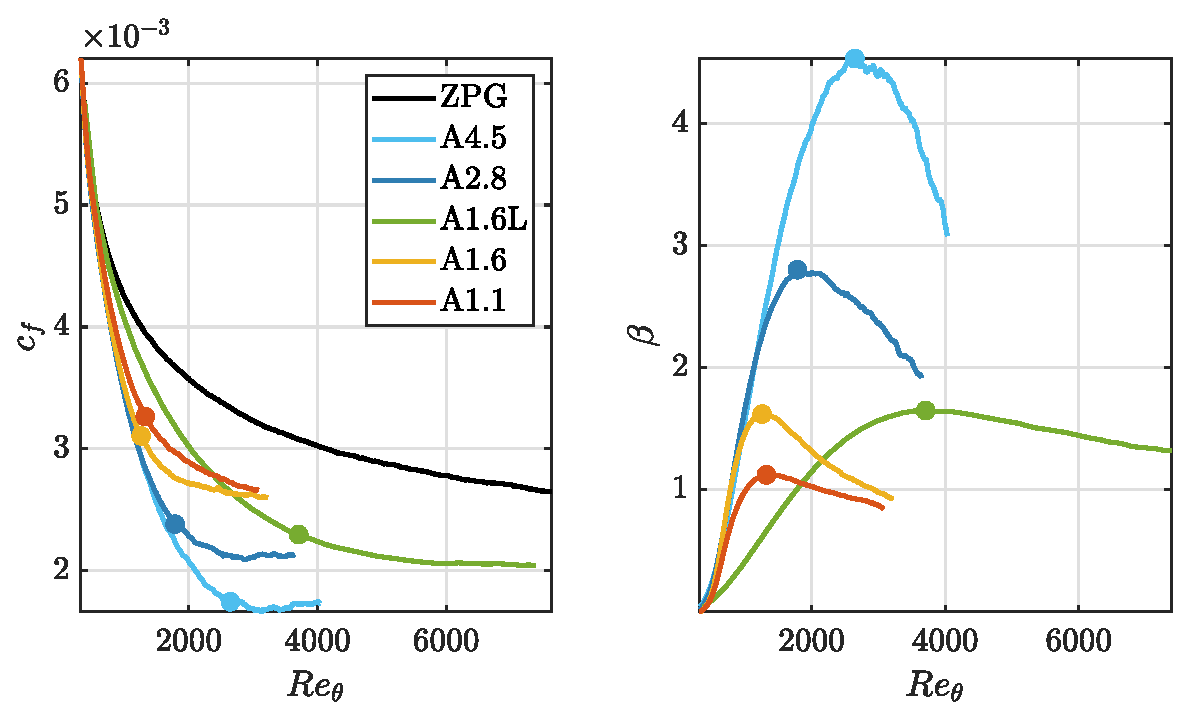
\includegraphics[width=0.48\textwidth]{01_overviewFP.eps}% Here is how to import EPS art
\caption{\label{fig:overviewFP} (Left) Skin-friction coefficient, denoted by $c_f$ and (right) Clauser pressure-gradient parameter, denote by $\beta$, for the flat-plate cases. The circles denote the location of maximum $\beta$.}
\end{figure}


\subsection{Airfoil}
The wing simulations considered in this work are well-resolved LES carried out with the code \textit{Nek5000}\cite{fischer2008nek5000}, which is based on the spectral-element method\cite{pate84} (SEM). 
The LES filter is based again on the same ADM-RT sub-grid model\cite{schl04} as for the flat-plate simulations, which was validated for this setup with DNS data\cite{hoss16} for the reference case at $Re_c=400,000$. The cases at ${\rm AoA}=5^\circ$ have been simulated using a conformal C-type mesh that extends up to a distance of $2c$ in each direction from the airfoil surface, and at least $0.2c$ in the spanwise direction\cite{vinu18b,atzo21b}. A RANS simulation provides boundary conditions at the inlet and upper and lower sides, and a local-stress outflow condition is used for the rear side of the domain\cite{dong14}. The mesh is designed using the wall-shear stress of RANS simulations so that the resolution in the turbulent region of the domain is approximately $(\Delta x^+,\Delta y^+,\Delta z^+) < (18,0.64-11,9)$. Note that the case with body-force damping is examined here for the first time, but it is analogous to a previous one with the same control at $Re_c=200,000$\cite{atzo21b}. The case at ${\rm AoA}=11^\circ$ is also examined here for the first time and uses a different setup, taking advantage of the recent implementation of adaptive mesh refinement in \textit{Nek5000}\cite{tanarro2020enabling}. In particular, the grid for the production case is obtained by progressively refining an initial mesh with \textit{h-type} refinement, \textit{i.e.} dividing spectral elements where it is needed, which is determined using a spectral error indicator\cite{mavr90}. The resulting mesh is non-conformal with a resolution in the turbulent region similar to that of the previous cases, allowing to use a much larger domain size that extents for $50c$, $40c$ and $0.6c$ in the horizontal, vertical and spanwise directions, respectively. The larger size of the domain reduces the impact of the boundary conditions and allows to properly describe the large turbulent structures in separation conditions. In all wing simulations, transition to turbulence is induced at a distance from the leading edge of $x/c=0.1$ using a random volume force with given intensity and length and time scales, implemented to simulate tripping devices in experiments\cite{schl12}. 

To provide an overview of these data sets, we show the skin friction and Clauser parameters as functions of the distance from the leading edge for all wing cases in Fig.~\ref{fig:overviewWIGN2},
\begin{figure}
\centering
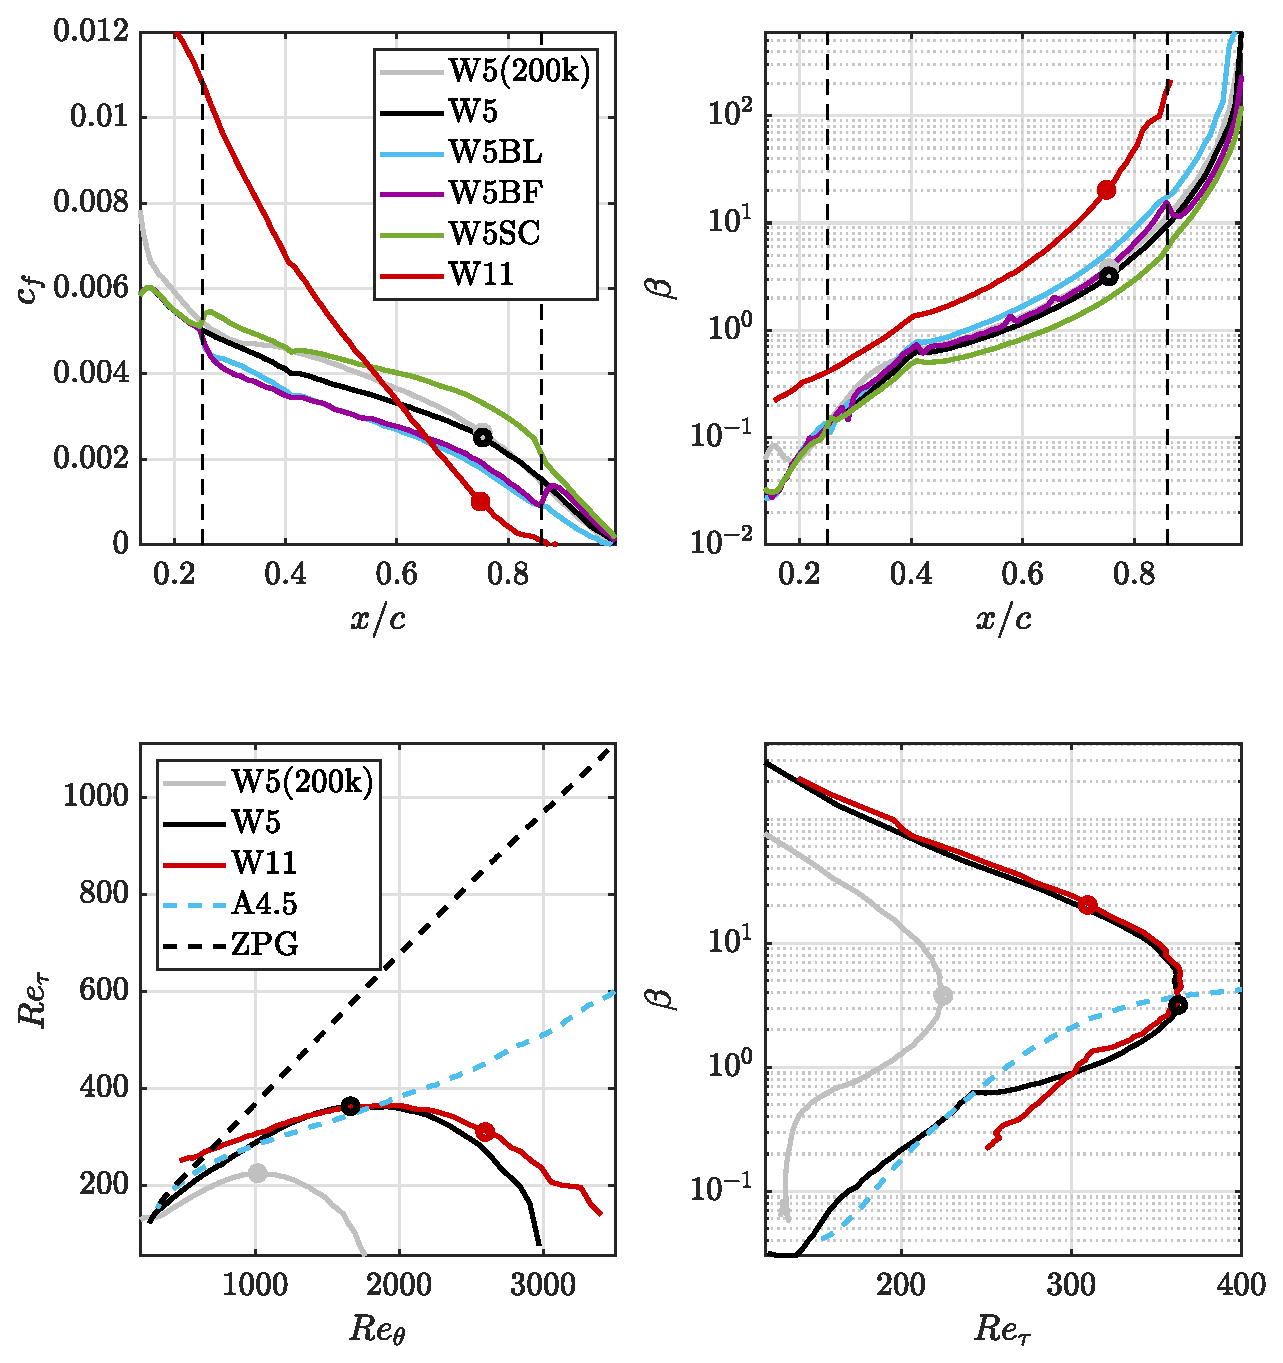
\includegraphics[width=0.48\textwidth]{01_overviewWING.eps}\caption{\label{fig:overviewWIGN2} (Top, left and right) Skin-friction coefficient and Clauser pressure-gradient parameter for the suction side of the NACA4412 cases, respectively. The dashed vertical lines denote the control region. (Bottom, left and right) Friction Reynolds number as a function of $Re_\theta$, and Clauser parameter as a function of $Re_\tau$, respectively. The circles in each plot denote location $x/c=0.75$.}
\end{figure}
together with $Re_\theta$ as a function of $Re_\tau$ and $\beta$ as a function of $Re_\tau$ for the cases without control and the flat-plate cases ZPG and A4.5. The local skin-friction decreases for all cases due to the progressively stronger APG. Uniform blowing and suction have approximately opposite effects, decreasing and increasing $c_f$, respectively. Body-force damping, as per design, causes a similar skin-friction reduction in the case with uniform blowing in the control region, but $c_f$ rapidly recovers further downstream (as previously observed on flate plate\cite{stro16}). The development of $\beta$ is very similar for the two cases W5(200k) and W5, which only differ for the value of $Re_c$. The streamwise evolution $Re_\tau$ in the wing cases is significantly affected by the pressure gradient. In internal-flow canonical cases, such as turbulent channel or pipe, and in ZPG TBLs, $Re_\tau$ is an indicator of the range of active scales and thus increases monotonically if the macroscopic Reynolds number increases. This still holds true for the APG flat-plate cases, even though $Re_\tau$ is reduced compared with the corresponding ZPG TBL. For the cases examined in the wing however, $Re_\tau$ is still increasing only up to a certain streamwise location, after which $u_\tau$ decreases faster than the growth of $\delta_{99}$, causing $Re_\tau$ to also decrease. 
 

\section{FIK identity for boundary layers}
The FIK identity is derived applying a triple integration by parts to the (partially) averaged Navier--Stokes equation\cite{fuka02}. This procedure results in a collection of terms, depending on the symmetry of the considered case. In the case of turbulent channel, which is periodic in both the streamwise and spawise directions, the total $c_f$ is expressed as:
\begin{equation}
    c_f = \frac{12}{Re_b} + 12 \int_0^2 (1-y) (-\overline{uv})\,{\rm d} y\,,
\end{equation}
where $Re_b=U_b H/\nu$ is the Reynolds number computed with bulk velocity $U_b$ and the full channel height $H$. 
In the case of turbulent boundary layers however, the flow is non-homogeneous in the streamwise direction and terms including derivatives in that direction do not vanish. Other identities, although derived with a different methodology, also result in similar collections of terms. In the present section, we summarize the terms of the FIK decomposition obtained from the conservative form of the averaged Navier--Stokes equations, which we referred to as ``standard'' formulation, and we consider a ``boundary-layer'' formulation. 

\subsection{Standard formulation}
The standard formulation of the FIK identity is derived applying a triple integration by parts to the averaged streamwise momentum conservation, which reads:
\begin{equation}
    \frac{\partial (U^2)}{\partial x} + \frac{\partial (UV)}{\partial y} = - \frac{\partial P}{\partial x} + \nu \left ( \frac{\partial^2 U}{\partial y^2} + \frac{\partial^2 U}{\partial x^2} \right ) + \frac{\partial \overline{uv}}{\partial y} + \frac{\partial \overline{u^2}}{\partial x}\,.
    \label{eq:NSx}
\end{equation}
This procedure results in the following identity:
\begin{equation}
    c_f = c^\delta_f + c^T_f + c^D_f + c^P_f\,,
\end{equation}
where each contribution is defined as:
\begin{eqnarray}
    c^\delta_f&=&4\frac{1-\delta_{99}/\delta^*}{Re_\delta}\,, \\
    c^T_f&=&-4\int_0^1 \int (1-\eta) \overline{uv}\,{\rm d}\eta\,, \\ 
    c^D_f&=&-2\int_0^1(1-\eta)^2 I_x\, {\rm d}\eta\,, \\
    c^P_f&=&-2\int_0^1 (1-\eta)^2 \frac{\partial P}{\partial x}\, {\rm d}\eta\,.
\end{eqnarray}
The first contribution directly takes into account the evolution of the boundary-layer thickness. The second contribution takes into account turbulent fluctuations. The third contribution includes all terms which would vanish in case of flows homogeneous in the streamwise direction, and the four contributions includes explicitly the pressure gradients. The multiplicative factors $(1-\eta)^n$ are a result of the integration by parts, and $\eta=y/\delta_{99}$ is the outer-scaled wall-normal location. When the FIK contributions are derived from the conservative form of the governing equations, the term $I_x$ is written as:
\begin{equation}
    I_x = \frac{\partial (U^2)}{\partial x} + \frac{\partial (\overline{u^2})}{\partial x} + \frac{\partial (UV)}{\partial y} - \frac{1}{Re_{\delta}} \frac{\partial^2 U}{\partial x^2}\,.
\end{equation}
Contributions $c^D_f$ can thus be expressed as the sum of four additional terms, as follows:
\begin{eqnarray}
    c^{D1}_f&=& -2\int^1_0(1-\eta)^2\, \frac{\partial (UU)}{\partial x}\, {\rm d}\eta, \\
    c^{D2}_f&=& -2\int^1_0(1-\eta)^2\, \frac{\partial \overline{u^2}}{\partial x}\, {\rm d}\eta, \\ 
    c^{D3}_f&=& -2\int^1_0(1-\eta)^2\, \frac{\partial UV}{\partial \eta}\, {\rm d}\eta  , \\
    c^{D4}_f&=&  -2\int^1_0(1-\eta)^2\, \left ( - \frac{1}{Re_\delta} \frac{\partial^2 U}{\partial x^2} \right )\, {\rm d}\eta.
\end{eqnarray}
Of these four contributions, $c^{D1}_f$ and $c^{D3}_f$, which are directly related with mean-velocity components, tend to be the most relevant of the non-homogeneous contributions.

\subsection{Boundary-layer formulation}
For the case of turbulent boundary layers, we propose a new formulation following three steps. The first step is simply to combine $c^{D1}_f$ and $c^{D3}_f$ using the continuity equation, which is equivalent to deriving the FIK identity from the convective form of the governing equations. In this case, the integrand of the non-homogeneous contribution, $c^D_f$, reads: 
\begin{equation}
    I^*_x = U\frac{\partial U}{\partial x} + \frac{\partial (\overline{u^2})}{\partial x} + V \frac{\partial U}{\partial y} - \frac{1}{Re_{\delta}} \frac{\partial^2 U}{\partial x^2}\,,
\end{equation}
resulting in different contributions from mean convection instead of $c^{D1}_f$ and $c^{D3}_f$. We denote the corresponding new contributions $c^{D1*}_f$ and $c^{D3*}_f$, respectively.


The second step is to consider together the new streamwise-convection term, $c^{D1*}_f$, and the pressure-gradient term, creating the following contribution:
\begin{eqnarray}
    c^{DP}_f &=& -2 \int_0^1 (1-\eta)^2 \left ( U \frac{\partial U}{\partial x} + \frac{\partial P}{\partial x} \right ) {\rm d} \eta\,.
\end{eqnarray}
This step is motivated with the following reasoning. In the free-stream region of the flow, outside the boundary layer, the Euler equation holds:
\begin{equation}
    U \frac{\partial U}{\partial x} = - \frac{\partial P}{\partial x}\,,
    \label{eq:Euler}
\end{equation}
This is also equivalent to the Bernoulli equation, 
\begin{equation}
    \frac 12 \rho U^2 +P = P_0\,,
    \label{eq:Bernoulli}
\end{equation}
which holds for points along streamlines in inviscid flows. In this expression, $P_0$ denotes the total pressure, which is constant along streamlines. The new contribution $c^{DP}_f$ is thus defined with the spirit of removing the apparent contributions to friction that are due to the development of the irrotational flow above the boundary layer. We name this new term ``dynamic-pressure contribution'' hereafter, as it describes the balance between the evolution of the dynamic pressure in the mean flow, $ 1/2 \partial(\rho U^2) / \partial x$, and the pressure gradient. 

The third step is to introduce a contribution which contains the mean spanwise vorticity, denoted by $\Omega_z=\partial V / \partial x -\partial U / \partial y$. This step is possible because, within the boundary layer, $\partial U / \partial y$ is by far the main term of $\Omega_z$. The new contribution related to wall-normal convection, $c^{D3*}_f$, is thus substituted by two new terms in the boundary-layer formulation: 
\begin{eqnarray}
    c^{D\Omega}_f &=& +2 \int_0^1 (1-\eta)^2 V \Omega_z \, {\rm d}\eta \,,\\
    c^{DV}_f &=& -2 \int_0^1 (1-\eta)^2 \left ( V \frac{\partial V}{\partial x} \right ) {\rm d} \eta\,.
\end{eqnarray}

The relation between the boundary-layer and standard FIK formulations can be summarized by the following identities between the contributions related to mean convection and pressure gradient:
\begin{eqnarray}
    &c^{DP}_f& = c^{D1*}_f + c^P_f = \frac 12 c^{D1}_f+c^P_f\,,\\
    &c^{D\Omega}_f& + c^{DV}_f = c^{D3*}_f  = \frac 12 c^{D1}_f + c^{D3}_f \,.
\end{eqnarray}


The same aggregation of contributions can be proposed for decompositions that have similar terms, \textit{i.e.\!} the RD decomposition if the non-homogeneous contribution is expressed in explicit form (see Appendix \ref{sec:appendix1}). Wenzel \textit{et al.}\cite{wenz22} used a similar approach to for the study of compressible TBLs to have better cancellations between the contributions of FIK identity derived from a double integration by parts. In their case, wall-tangential convection and pressure gradient are also considered together, but the different form of the Bernoulli equation for compressible flows makes the interpretation of the resulting spatial-development term less intuitive.


Even though defining the upper bound of integration is a critical point in the application of skin-friction decompositions to APG TBLs, we do not investigate this point further in the present paper. We assume that a definition of the boundary-layer thickness is provided and that it is consistent with the flow development. The results shown hereafter are obtained using $\delta_{99}$ based on the diagnostic scaling, as mentioned in \S2. Previous studies reported only a small dependency of contributions for small changes of $\delta_{99}$, as expected from the shape of the integration pre-factor and the properties of the flow\cite{atzo21}. Furthermore, $c^{DP}_f$ is automatically negligible beyond the edge, which makes the boundary-layer formulation even less sensitive than the standard one. It is also worth mentioning that Griffin \textit{et al.}\cite{grif21} recently proposed a method to identify $\delta_{99}$ based on a comparison between the mean velocity in the TBL and the expected velocity from the irrotational free-stream flow. This method uses a condition naturally similar to the definition of $c^{DP}_f$ and it gives equivalent results to the one used in the present paper with an equivalent definition of the edge. We can then state that the FIK identity is used in this form to study the balance of contributions in the domain region within the boundary layer. 



\section{Results}
In this section, we examine the FIK contributions for a selected set of pressure-gradient conditions. We focus on how the boundary-layer formulation can improve the description of both pressure-gradient and control effects, and on how the new dynamic-pressure contribution can be used to identify different flow regimes.

\subsection{APG effects over the flat plate}

Firstly, we compare the canonical zero-pressure-gradient TBL and the adverse-pressure-gradient TBL in case A1.6L, which exhibits moderate values of $\beta$. Fig.~\ref{fig:contributionsFP} shows the skin-friction contributions and the relative skin-friction contributions in both cases and for both formulations as functions of $Re_\theta$. The values of the relative contributions for three selected locations are reported in Table~\ref{tab:contributionsFP}. The relative contributions are normalized with the total $c_f$ of each case, so that their sum is $1$. Note that the qualitative development of relative contributions may differ from that of absolute contributions, depending on the rate of the change of $c_f$. For example, a relative contribution will still increase even when the corresponding absolute contribution decreases, if $c_f$ decreases faster. 
\begin{figure}
\centering
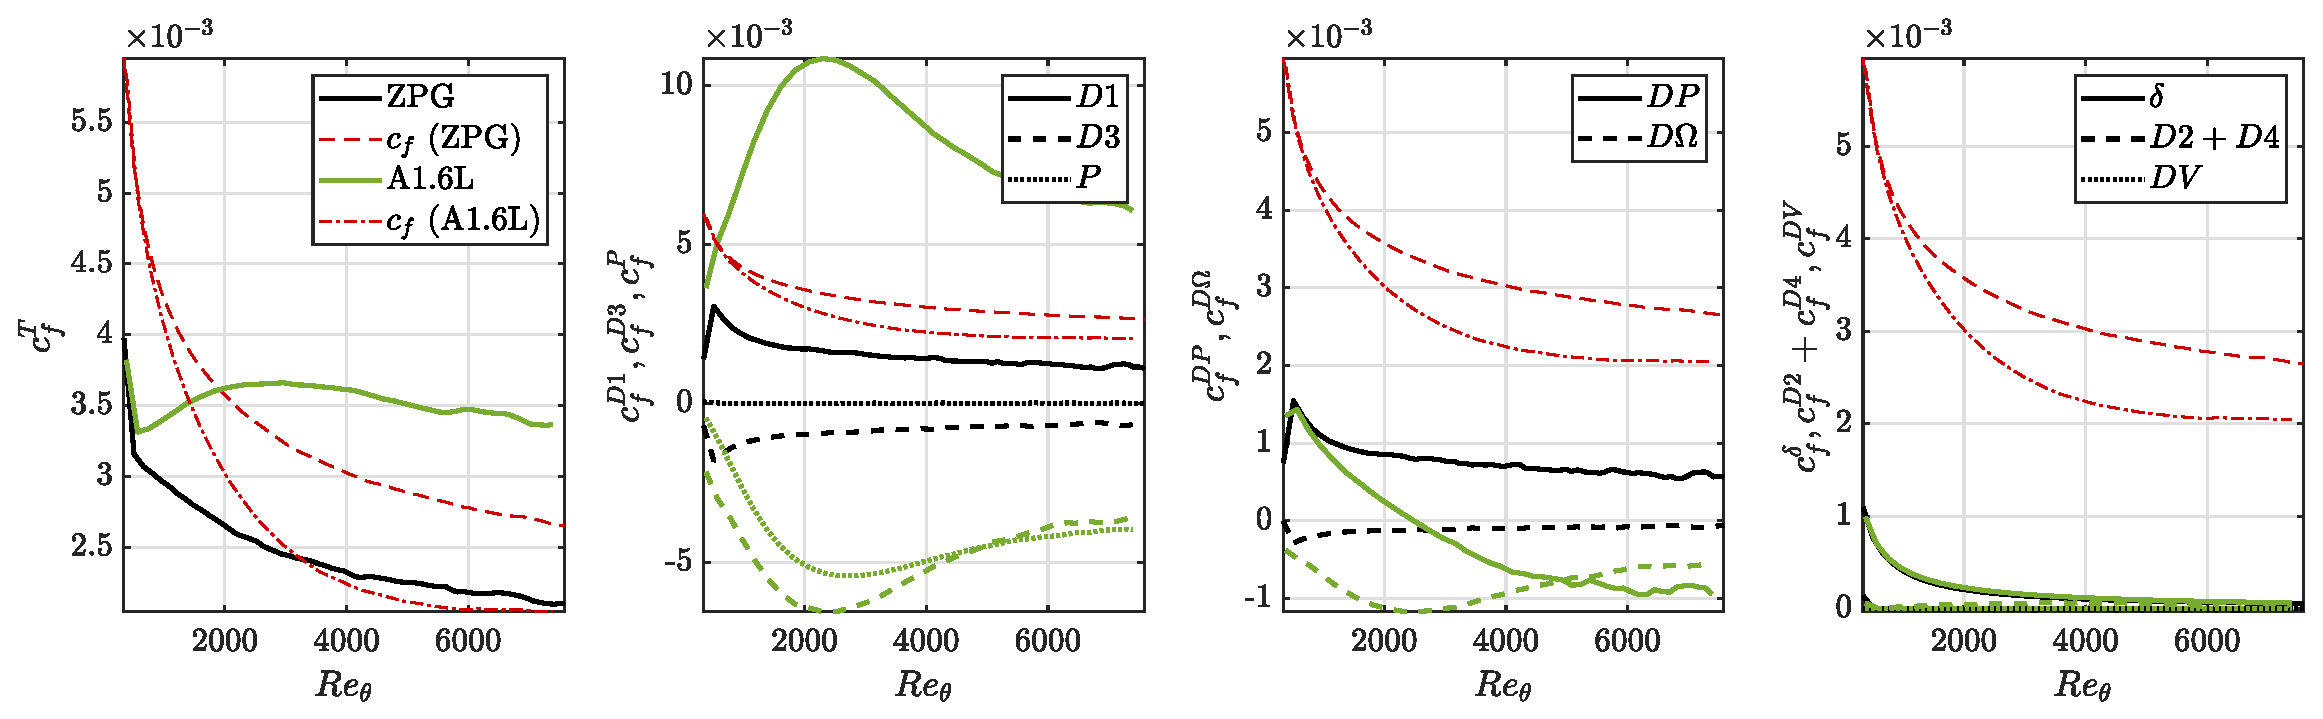
\includegraphics[width=0.98\textwidth]{02_absolute_contributions.eps}\\% Here is how to import EPS art
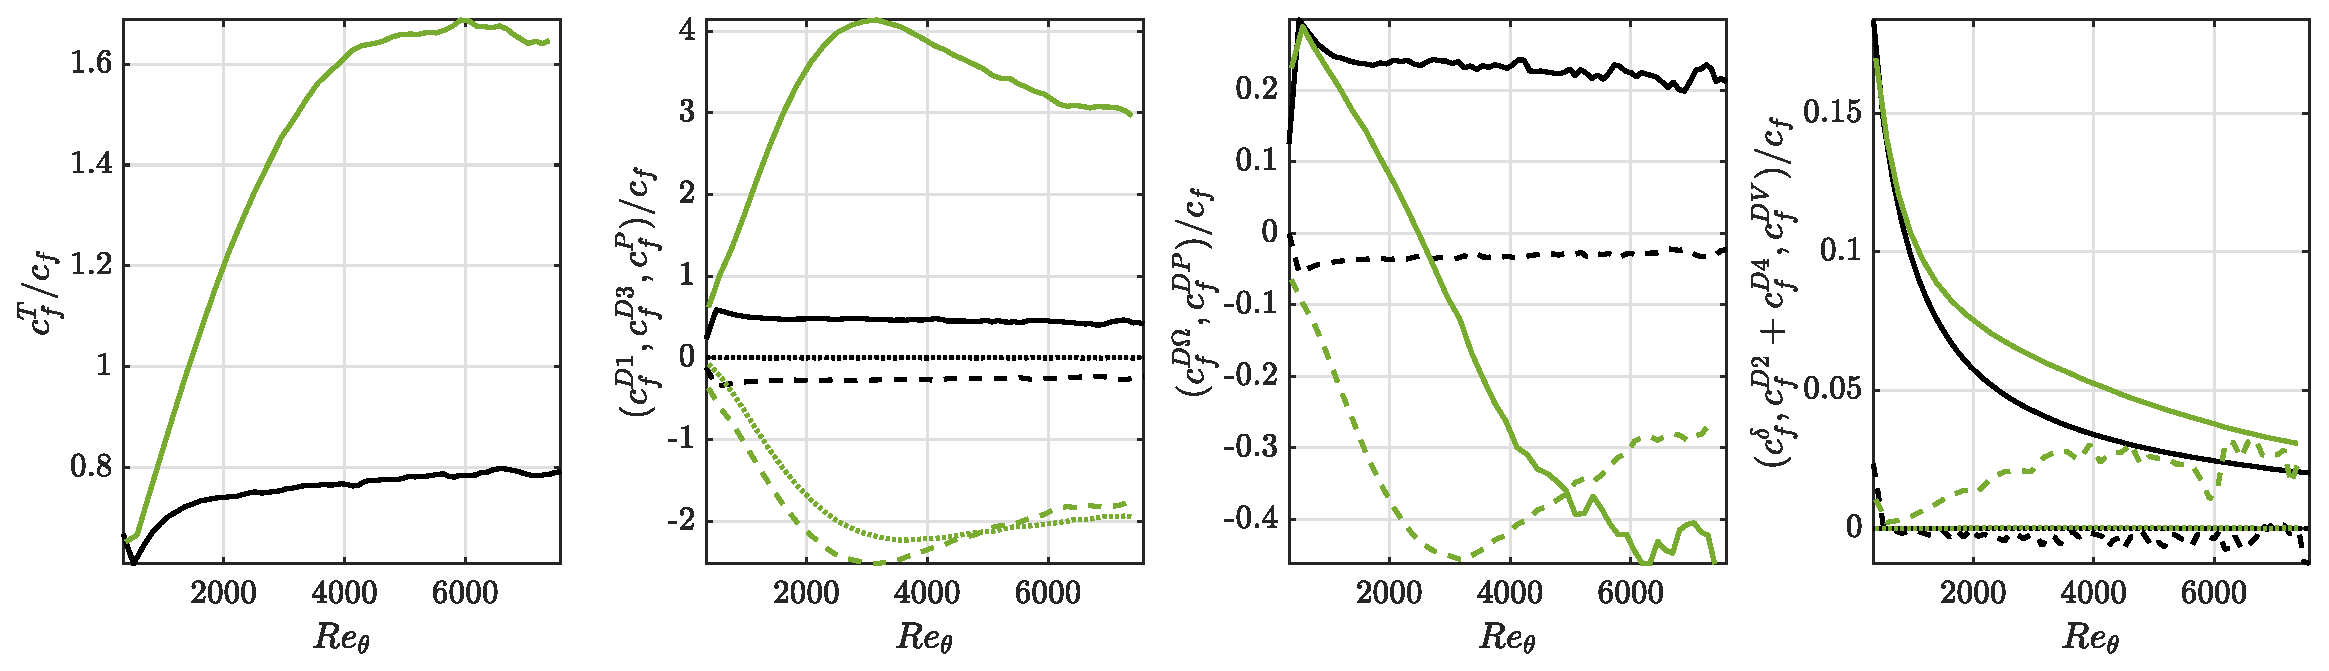
\includegraphics[width=0.98\textwidth]{02_relative_contributions.eps}% Here is how to import EPS art
\caption{\label{fig:contributionsFP} (Top row) Contributions and (Bottom row) relative contributions to the skin friction for cases ZPG and A1.6L, calculated using both the standard and boundary-layer FIK formulations.}
\end{figure}
\begin{table}
\caption{\label{tab:contributionsFP} Most relevant skin-friction contributions for the standard and boundary-layer formulation of the FIK identity in the ZPG and A1.6L cases at selected locations. The last line shows the sum of the contributions reported here, neglecting the remaining terms. Note that $c^{D1}_f+c^{D3}_f+c^{P}_f=c^{DP}_f+c^{D\Omega}_f+c^{DV}_f$, and $c^{DV}_f$ is always negligible.}
\centering
\begin{tabular}{ccccccc}
\hline \hline
 &\multicolumn{3}{c}{ZPG}&\multicolumn{3}{c}{A1.6L}\\ \hline
$\beta$ & $0$ & $0$ & $0$ & $1.2$ & $1.6$ & $1.4$ \\
$Re_\theta$ & $2000$ & $4000$ & $6000$ & $2000$ & $4000$ & $6000$ \\
$Re_\tau$ & $680$ & $1300$ & $1800$ & $530$ & $850$ & $1200$ \\ \hline
$c^T_f/c_f$ & $\bm{0.74}$ & $\bm{0.77}$ & $\bm{0.78}$ & $1.20$ & $1.60$ & $1.70$ \\ \hline
$c^{D1}_f/c_f$ & $0.48$ & $0.48$ & $0.45$ & $\bm{3.50}$ & $\bm{3.90}$ & $\bm{3.20}$ \\
$c^{D3}_f/c_f$ & $-0.27$ & $-0.27$ & $-0.25$ & $-2.10$ & $-2.40$ & $-1.90$ \\
$c^{P}_f/c_f$ & $0$ & $0$ & $0$ & $-1.70$ & $-2.20$ & $-2.00$ \\ \hline
$c^{DP}_f/c_f$ & $0.24$ & $0.24$ & $0.22$ & $0.08$ & $-0.28$ & $-0.42$ \\
$c^{D\Omega}_f/c_f$ & $-0.04$ & $-0.03$ & $-0.03$ & $-0.38$ & $-0.42$ & $-0.30$ \\ \hline
$\sum/c_f$ & $0.94$ & $0.97$ & $0.98$ & $0.91$ & $0.92$ & $0.96$  \\
\hline \hline
\end{tabular}
%  
\end{table}


When compared against the ZPG case, APG TBLs exhibit a faster decrease of $c_f$ as the boundary-layer develops, which is also matched by a qualitative change in the FIK contributions. The turbulent-fluctuations contribution, $c^T_f$, which has the same expression in both FIK formulations, progressively decreases in the ZPG case but it increases in the streamwise region that approximately coincides with the increase of $\beta$. 


Already for the ZPG case, the contributions are significantly different between the standard and boundary-layer formulations. In particular, in the standard formulation, both $c^{D1}_f$ and $c^{D3}_f$ have not-negligible values, albeit lower than $c^T_f$. In the boundary-layer formulation however, $c^{D\Omega}_f$ only reaches low values, \textit{e.g.\!} $-3\%$ of $c_f$ at $Re_\theta=4,000$ instead of $-27\%$ of the corresponding $c^{D3}_f$. This immediately clarifies that wall-normal convection is actually negligible in the ZPG case. The boundary-layer formulation then shows that skin friction is generated in ZPG TBL mainly as a combination of the turbulent fluctuations and the dynamic-pressure contributions.


The three contributions $c^{D1}_f$, $c^{D3}_f$, and $c^{P}_f$ are the more relevant ones for the standard FIK formulation in the APG case. The streamwise-convection contribution, $c^{D1}_f$, is positive, while the wall-normal convection and pressure gradient contributions, $c^{D3}_f$ and $c^{P}_f$, respectively, are negative. All these terms have absolute values that are relatively high. In particular, $c^{D1}_f$ reaches up to $4$ times the total $c_f$ in case A1.6L. These contributions are also higher than $c^T_f$ for the APG case at every $Re_\theta$ and $\beta$. The streamwise development of the standard FIK contributions also suggests that a change of regime is occurring at a certain $Re_\theta$ slightly above $2,000$, where the absolute values of $c^{D1}_f$, $c^{D3}_f$, and $c^{P}_f$ start to decrease. However, it is not immediately possible to identify whether this change of regime modifies the balance among the various terms. In the boundary-layer formulation, on the other hand, $c^{DP}_f$ and $c^{D\Omega}_f$ are lower than $c^T_f$ and the sign of $c^{DP}_f$ immediately describes the balance between streamwise convection and pressure gradient. In case A1.6L, this term is initially positive but it decreases and changes sign at  $Re_\theta\approx2,500$. At the same time, $c^{D\Omega}_f$ is always negative, it initially decreases up to $Re_\theta\approx2,500$, and then it increases farther downstream. 


Of the reaming terms, the most relevant is $c^\delta_f$, but this contribution is always decreasing for both ZPG and APG cases as the Reynolds number increases. On the other hand, $c^{D4}_f$ is slightly increasing but still remains very low. Overall, these terms are all progressively less relevant at higher Reynolds number, so that the sum of the larger ones accounts for \textit{e.g.} $98\%$ and $96\%$ of $c_f$ at $Re_\theta=6,000$ for ZPG and A1.6L, respectively. This result is the same for both formulations, due to the extremely low values of $c^{DV}_f$. 


We now focus on the region of rapidly increasing $\beta$ before $Re_\theta\approx3,000$ to discuss more in detail the behaviour of the new contributions $c^{DP}_f$ and $c^{D\Omega}_f$, also considering the other flat-plate cases. Compared to A1.6L, these cases exhibit a higher rate of change of $\beta$ in the aforementioned region. For instance, case A1.6 reaches $\beta=1.6$ at $Re_\theta=1,260$ while case A1.6L reaches the same value at $Re_\theta=3,700$. The faster increase of $\beta$ results in more pronounced APG effects, as TBLs tend to be less sensitive to pressure gradient at higher Reynolds numbers. This is firstly illustrated by a higher $c^T_f$ relative contribution, which increases approximately up to the location of maximum $\beta$ (Fig.~\ref{fig:contributionsAPG}, left). However, it is the behaviour of $c^{DP}_f$ and $c^{D\Omega}_f$ that exhibits more important differences for different developments of $\beta$ (Fig.~\ref{fig:contributionsAPG}, right).
\begin{figure}
\centering
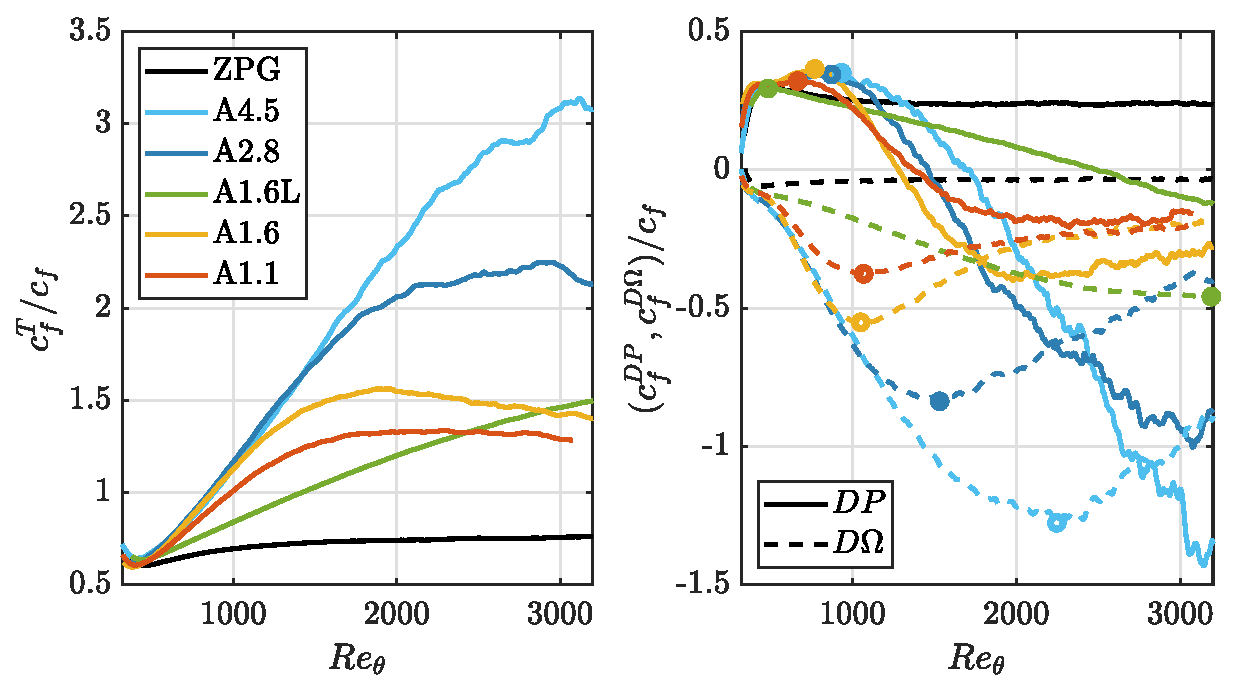
\includegraphics[width=0.48\textwidth]{03_CDP_FP.eps}% Here is how to import EPS art
\caption{\label{fig:contributionsAPG} Relative contributions related to (left) turbulent fluctuations and (right) dynamic pressure and wall-normal convection for all flat-plate cases.}
\end{figure} 
The relative contribution of the dynamic pressure $c^{DP}_f/c_f$ increases over a longer streamwise region in the cases with faster growth of $\beta$. At the same time, $c^{D\Omega}_f/c_f$ reaches a lower value in these cases than in A1.6L. In all flat-plate cases, $c^{DP}_f$ decreases and eventually changes sign while $c^{D\Omega}_f$ remains negative but increases at higher $Re_\theta$ when pressure-gradient effects are less strong. To better describe the streamwise evolution of the dynamic-pressure and vorticity-convection contributions, we report in Table~\ref{tab:maxLocation} two indicators of the development of $\beta$, \textit{i.e.\!} the location of maximum $\beta$ and the location of the maximum rate of change of $\beta$, together with the position and value of the maximum of $c^{DP}_f/c_f$ and the minimum of $c^{D\Omega}_f/c_f$. The rate of change of $\beta$ is defined as ${\rm d} \beta / {\rm d} x$ and it is considered here to give a qualitative indication of the streamwise evolution of $\beta$.


\begin{table}
\caption{\label{tab:maxLocation} Locations of maximum $\beta$, maximum rate of change of $\beta$, maximum $c^{DP}_f/c_f$ and minimum $c^{D\Omega}_f/c_f$, and values of $c^{DP}_f/c_f$ and $c^{D\Omega}_f/c_f$ and the location of their extrema.}
\centering
  \fontsize{8.0pt}{12.25pt}\selectfont
  \addtolength{\tabcolsep}{-2pt}
\begin{tabular}{cccccc}
\hline \hline
 &A1.1&A1.6&A2.8&A4.5&A1.6L\\ \hline
$Re_\theta({\rm max}[\beta])$ & $1300$ & $1300$ & $1800$ & $2600$ & $3700$ \\
$Re_\theta({\rm max}[{\rm d} \beta/{\rm d} x])$ & $690$ & $710$ & $880$ & $1200$ & $1400$ \\ \hline
$Re_\theta({\rm max}[c^{DP}_f/c_f])$ & $670$ & $770$ & $870$ & $930$ & $490$ \\
${\rm max}[c^{DP}_f/c_f]$ & $0.32$ & $0.37$ & $0.35$ & $0.35$ & $0.29$ \\ \hline
$Re_\theta({\rm min}[c^{D\Omega}_f/c_f])$ & $1100$ & $1000$ & $1500$ & $2200$ & $3200$ \\
${\rm min}[c^{D\Omega}_f/c_f]$ & $-0.38$ & $-0.55$ & $-0.84$ & $-1.30$ & $-0.46$ \\
\hline \hline
\end{tabular}
%  
\end{table}


 It appears that $c^{DP}_f$ is particularly sensitive to the variation of pressure-gradient conditions, as shown by the following observations. On the one hand, for cases A1.1, A1.6, and A2.8, the location of highest ${\rm d} \beta / {\rm d} x$ is close to that of the maximum of $c^{DP}_f$. For case A4.5, the maximum of $c^{DP}_f/c_f$ appears upstream than that of ${\rm d} \beta / {\rm d} x$, and in fact in a location similar to that of case A2.8. For case A1.6L, the location of maximum $c^{DP}_f$ is even more upstream than the location of maximum ${\rm d} \beta / {\rm d} x$. In all cases, the change from a regime of increasing $c^{DP}_f/c_f$ to a regime of decreasing $c^{DP}_f/c_f$ is thus not related with location of maximum $\beta$, but rather with how fast $\beta$ is increasing. Decreasing after its maximum, $c^{DP}_f$ eventually becoming negative. The wall-normal convection of vorticity adapts to changes in the pressure conditions more slowly than $c^{DP}_f$. This contribution is always negative and decreases up a location which is slightly upstream that of the maximum of $\beta$, after which increases approaching zero from below. 
 
 
 The results analysed in this section show that there are different mechanisms that lead to the faster rate at which $c_f$ decreases in APG cases with respect to the ZPG TBL, as illustrated by the balance between various skin-friction contributions. This fact is a direct consequence of the different sensitivity of the contributions to change in pressure conditions, in particular in the case of $c^{DP}_f$ and $c^{D\Omega}_f$.

\subsection{APG effects over the airfoil suction side}
We now turn our attention to the TBL developing on the suction side of the wing profile. The TBLs on the wing profiles differ significantly from the ones analyzed so far because they eventually reach higher values of $\beta$ and because $\beta$ is monotonically increasing. These particular pressure-gradient conditions result in the entirety of the wing boundary layer to correspond to the portion of the flat-plate cases where $\beta$ is also increasing, at least to some extent. The turbulent-fluctuation, dynamic-pressure and vorticity-convection contributions and the corresponding relative contributions for streamwise region $0.4<x/c<0.8$ are shown in Fig.~\ref{fig:contributionsWing}, together with those of case A4.5, which is the flat-plate case that reaches the highest value of $\beta$. 

\begin{figure}
\centering
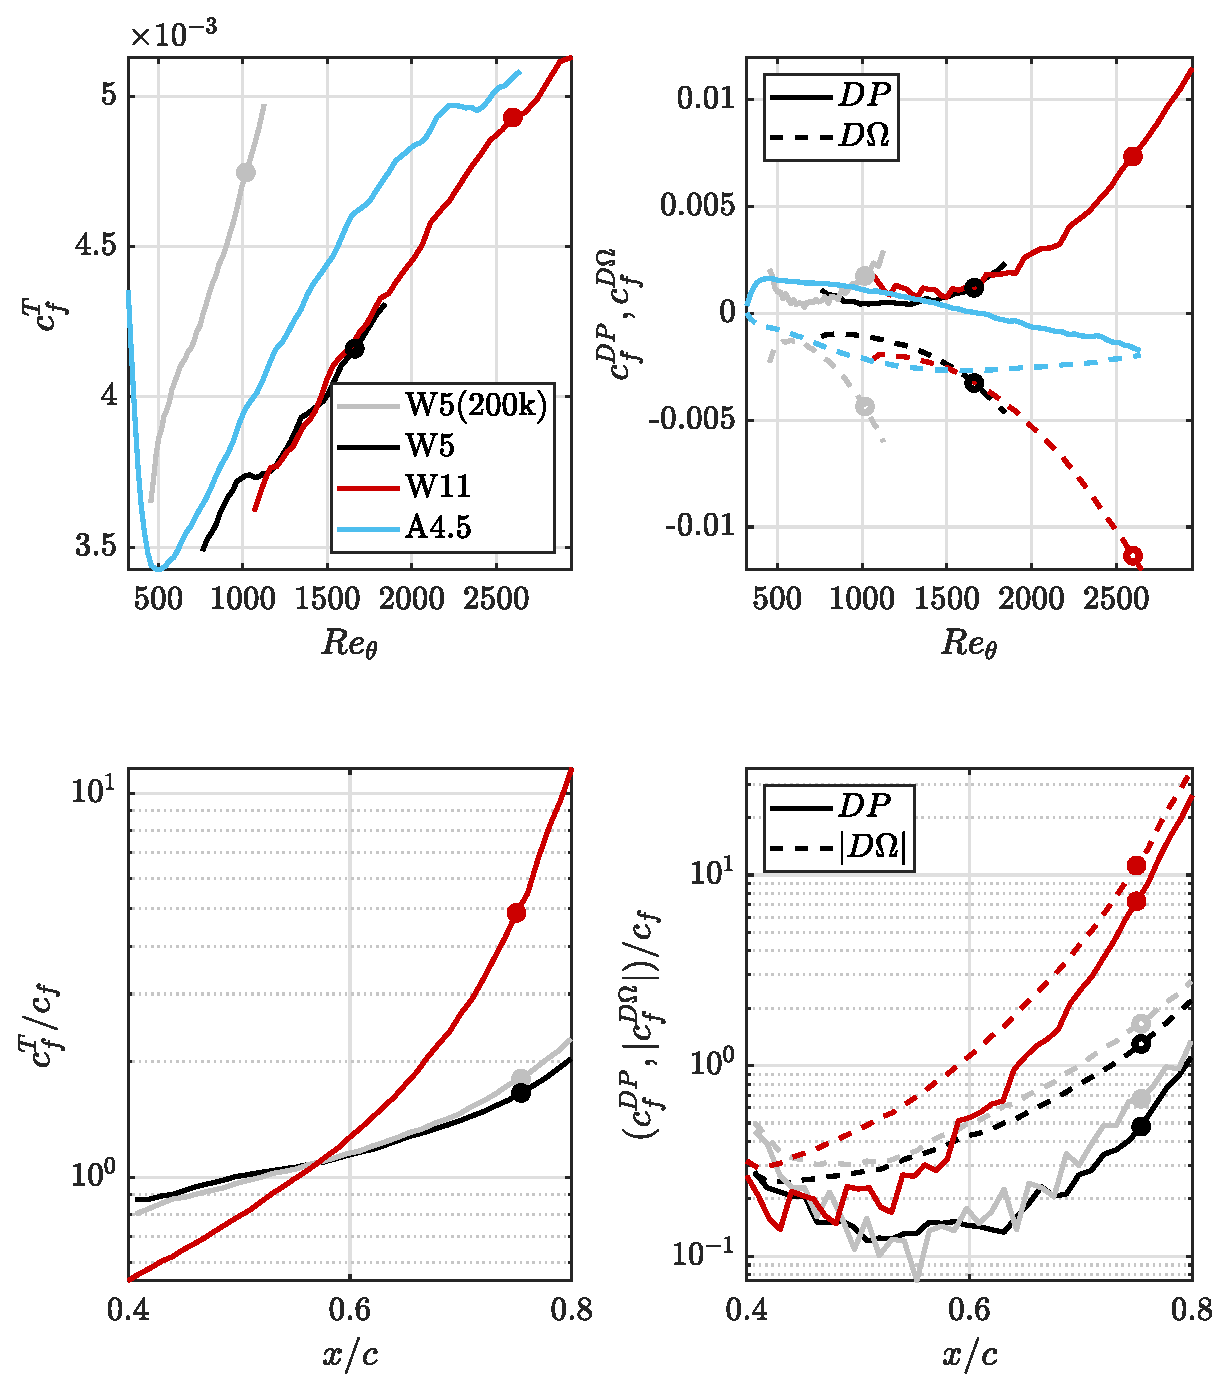
\includegraphics[width=0.48\textwidth]{04_CDP_WING.eps}
\caption{\label{fig:contributionsWing} (Top) Most relevant contributions for boundary-layer FIK formulation in cases W5(200k), W5, W11, and A4.5 as functions of $Re_\theta$ and (bottom) corresponding relative contributions for the wing cases as functions of $x/c$ (note that $|c^{D\Omega}_f|$ is shown here for clarity). Only the streamwise region $0.4<x/c<0.8$ is shown for the wing cases and only the region up the maximum value of $\beta$ for case A4.5. }
\end{figure}


The increasing value of $\beta$ leads to an also increasing $c^T_f$ contribution for all the wing cases, while the streamwise development of the dynamic-pressure and vorticity-convection contributions is more complex. Contrary to the flat-plate cases, $c^{DP}_f$ always remains positive, although it initially decreases in the first portion of the wing profile. This is a region of relatively slow rate of change of $\beta$. In the same region, $c^{D\Omega}_f$ increases its value (\textit{i.e.\!} reduces its absolute value). Further downstream however, both $c^{DP}_f$ and $c^{D\Omega}_f$ rapidly increase in absolute values and, in case W11, eventually reach more than $10$ times the value of $c_f$ in the region considered here. The comparison between the three wing cases shows how the more intense APG in case W11 corresponds to a faster increase of the contributions than in case W5. Similarly, the lower Reynolds number in case W5(200k) also causes APG effects to be more pronounced than in case W5, although just slightly. Examining these results allows to draw a more precise comparison between the flat-plate and the wing cases. In particular, it is the second portion of the suction side that corresponds to the first portion of the flat-plate cases. The first portion of the suction side is instead more similar to region in the flat plate downstream the maximum rate of change of $\beta$. A distinction from the flat-plate cases is the fact that the streamwise evolution of $c^{D\Omega}_f$ is observed to immediately match that of $c^{DP}_f$. This is in contrast to what was observed before, where the evolution of $c^{DP}_f$ anticipated that of $c^{D\Omega}_f$. Such a difference may be caused to the more abrupt evolution of the pressure condition over the airfoil suction side.


To give a more precise indication of the relative values of the contributions, we report the most-relevant terms at $x/c=0.75$ in Table~\ref{tab:contributionsWING}, together with those from case A4.5 at the location with same $Re_\theta$ of case W5 at $x/c=0.75$. The relatively low Reynolds number causes contributions $c^T_f$, $c^{DP}_f$, and $c^{D\Omega}_f$ to account for a relatively lower portion of the total $c_f$ with the respect to remaining terms than in the locations previously considered in Table\ref{tab:contributionsFP}. The streamwise development of $c^\delta_f$, $c^{D4}$, and $c^{D2}_f$, however, follow the same general trend as that in case A1.6L and is not shown here. The comparison between relative contributions in cases W5 and A4.5 illustrates the difference between the two flow regimes. At the considered locations, $\beta$, $Re_\theta$, and $Re_\tau$ have very similar values, and $\beta$ is still increasing in both cases (the maximum value of $\beta$ in case A4.5 is at $Re_\theta=2,600$). Nevertheless, $c^{DP}_f$ is positive and accounts for $50\%$ of $c_f$ in case W5, while it is negligible in case A4.5 at this location. At the same time, the absolute value of $c^T_f/c_f$ is higher in case A4.5 and that of $c^{D\Omega}_f/c_f$ is lower. These results constitute an additional confirmation of the relevance of history effects in APG TBLs. The comparison between cases W5 and W11 shows that the mechanism by which $c_f$ is progressively reduced in the case of very intense APG separation is the cancellation of progressively higher contributions, where the negative term $c^{D\Omega}_f$ has the highest rate of change. 

\begin{table}
\caption{\label{tab:contributionsWING}Most-relevant skin-friction contributions for the boundary-layer formulation of the FIK identity at selected $Re_\theta$ and streamwise locations on the suction side of the airfoil and in case A4.5. The last line shows the sum of the contributions reported here, neglecting the remaining terms.}
\centering
\begin{tabular}{ccccc}
\hline \hline
 &W5(200k)&W5&{W11}&A4.5\\ \hline
$x/c$ & $0.75$ & $0.75$ & $0.75$ & $-$ \\
$\beta$ & $3.8$ & $3.2$ & $20.0$ & $3.4$ \\
$Re_\theta$ & $1000$ & $1700$ & $2600$ & $1700$ \\
$Re_\tau$ & $220$ & $360$ & $310$ & $350$ \\ \hline
$c^T_f/c_f$ & $1.8$ & $1.7$ & $4.9$ & $2.0$ \\ \hline
$c^{DP}_f/c_f$ & $0.7$ & $0.5$ & $7.3$ & $\approx0$ \\
$c^{D\Omega}_f/c_f$ & $-1.7$ & $-1.3$ & $-11.0$ & $-1.1$ \\ \hline
$\sum/c_f$ & $0.80$ & $0.83$ & $0.86$ & $0.86$   \\
\hline \hline
\end{tabular}
%  
\end{table}

\subsection{Flow regimes in TBL}
Our observations on the skin-friction contributions for the boundary-layer FIK formulation can be summarized considering two different aspects. The first one is the sign of the dynamic-pressure contribution, $c^{DP}_f$, and the second is how the rate of change of the contributions correlates with that of $c_f$.


Due to its definition, $c^{DP}_f$ is zero in the case of an irrotational flow, where the total pressure $P_0$ is constant, following the Bernoulli equation. In the ZPG boundary layer, \textit{i.e.\!} $\partial P / \partial x=0$, the streamwise derivative of the dynamic pressure is negative and, due to the change of sign in the integration, $c^{DP}_f$ is positive. In the APG case, $\partial P / \partial x$ is positive, and we observed that $c^{DP}_f$ can be both positive and negative. A positive $c^{DP}_f$ is caused by $|U (\partial U/\partial x)|>\partial P / \partial x$, \textit{i.e.\!} a (negative) rate of change of the dynamic pressure in the boundary layer that is faster than that of the corresponding irrotational flow in that pressure condition. This condition implies a decrease of the total pressure. To the contrary, $c^{DP}_f<0$ is cause by $|U (\partial U/\partial x)|<\partial P / \partial x$, \textit{i.e.\!} a rate of change of the dynamic pressure that is slower than that of the corresponding irrotational flow, implying an increase of the total pressure. In the data set considered in this work, a positive dynamic-pressure contribution is connected with a rapidly increasing value of $\beta$, while a negative contribution is connected with almost uniform or decreasing $\beta$. 


The rate of change of the different $c_f$ contributions is of particular interest for possible implications in the study of separation. In principle, a reduction of $c_f$, eventually leading to mean separation ($c_f=0$), could be reached either by a progressive decrease in the absolute value of all the different contributions, or by cancellation of terms with opposite sign. In the first case, the rate of the change of $c_f$ will coincide with that of the contribution with the lowest rate of change, and the relative weight of the other contributions will remain approximately constant or decrease. This is in fact what is observed in the ZPG case, where the local $c_f$ progressively decreases solely per effect of the Reynolds number as the boundary layer develops. In the second case (observed in APGs), contributions of different signs may have different rates of change, and the relative contributions will eventually diverge at $c_f=0$. This is observed under certain pressure-gradient conditions; in fact, it is possible to identify three different regimes in the APG data set that we examined. 


In the first regime, $c^{DP}_f$ is positive and both $c^T_f$ and $c^{DP}_f$ are increasing in absolute and relative values, but $c^{D\Omega}_f$, which is negative, is decreasing at a higher rate, causing a rapid decrease of $c_f$. This regime is associated with a rapidly increasing value of $\beta$, and it is what we observed for case W11, where separation occurs, as well as for cases W5(200k) and W5, which have similar pressure-gradient conditions. In the second regime, $c^{DP}_f$ is negative and $c^{DP}_f$ and $c^{T}_f$ are both decreasing, while $c^{D\Omega}_f$ is increasing (\textit{i.e.} its absolute value decreases). This regime is observed at high Reynolds number in case A1.6L and it seems to coincide with the near-equilibrium state\cite{Bobke2017}. Despite the fact that $\beta$ is still positive, the state of the boundary layer in this regime is quite similar to that of the ZPG case, in the sense that $c_f$ has a relatively low rate of change and cancellation between terms play a minor role in determining its decrease. The third regime is an intermediate state. In this regime, $\beta$ can be either increasing or decreasing, and $c^{DP}_f$ can be either positive or negative, but it decreases. The qualitative behaviour of the most relevant contributions for the various regimes are summarized in Table~\ref{tab:regimes} and Fig.~\ref{fig:test}. 


\begin{table}
\caption{\label{tab:regimes}Summary of the trends of the main skin-friction contributions for the boundary-layer FIK formulation in the ZPG case and in the three regimes identified in APG TBLs.}
\centering
\begin{tabular}{cccc}
\hline \hline
 & $c^T_f$ & $c^{DP}_f$ & $c^{D\Omega}_f$\\ \hline
ZPG & decreasing & decreasing & decreasing \\
APG: near equilibrium & decreasing & decreasing & increasing \\
APG: towards separation & increasing & increasing & decreasing \\
APG: intermediate & increasing & decreasing & (both) \\
\hline \hline
\end{tabular}
%  
\end{table}


\begin{figure}
\centering
\includegraphics[width=0.48\textwidth]{Test.png}
\caption{\label{fig:test} Sketch of the trends of the main skin-friction contributions for the boundary-layer FIK formulation in the ZPG case and for APG near-equilibrium and towards separation (not to scale). }
\end{figure}


\subsection{Control effects over the airfoil suction side}
Lastly, we examine the effects of uniform blowing, body-force damping, and uniform suction on the FIK contributions for both the standard and boundary-layer formulations, to discuss how the latter can improve the description of control applied to TBLs. We focus our attention on streamwise location $x/c=0.75$ of the suction side of the airfoil, which is the same considered before.


The relative control effects on the standard contributions are reported in Table~\ref{tab:FIKcontrol}. These quantities are defined as the difference between the absolute contributions in the control and uncontrolled cases, normalized with the total $c_f$ of the uncontrolled case. According to this definition, the sum of all relative control effects is the total relative change of $c_f$ with respect to the uncontrolled case, which is denoted by $\Delta c_f/c_f^*$. This definition allows to identify which contribution is more relevant to describe the control effect on $c_f$. As already discussed\cite{atzo21b}, control effects on the standard FIK contributions are quite complex, which is in part a consequence of the very high absolute values of each term already in the uncontrolled case. Uniform blowing and uniform suction achieve skin-friction reduction and increase, respectively, through the wall-normal contribution $c^{D3}_f$. The term $c^{D1}_f$ however is increased by an amount that is almost as high as the decrease of $c^{D3}_f$ in uniform blowing, while the reduction of $c^P_f$ is not negligible either (uniform suction causes similar changes in the opposite directions). In fact, the modification of the pressure-gradient contribution for both blowing and suction is higher than the total change of $c_f$, and even higher than the sum of the two mean-convection contributions $c^{D1}_f$ and $c^{D3}_f$. This result may raise the question of whether the modification of pressure conditions above the boundary layer due to the control is in fact ultimately responsible for the change of drag, rather than a modification of momentum transfer within the boundary layer. The results for body-force damping are even more counter-intuitive. In particular, the term closely connected with the $c_f$ reduction appears to be $c^{D1}_f$, which is reduced by more than twice the reduction of $c^T_f$. At the same time, $c^{D3}_f$ and $c^{P}_f$ are increased as a result of this control by non-negligible amounts, a fact that also does not have a clear interpretation.


\begin{table}
\caption{\label{tab:FIKcontrol}Relative effects of the control on the skin-friction contributions in the standard FIK formulation and at $x/c=0.75$. The total skin friction of the reference case, W5, is denoted by $c_f^*$.}
\centering
\begin{tabular}{cccc}
\hline \hline
 &W5BL& W5BF & W5SC\\  \hline
$\Delta c^T_f/c_f^*$ & $+0.17$ & $-0.25$ & $-0.21$ \\   \hline
$\Delta c^{D1}_f/c_f^{*}$ & $+1.70$ & $\bm{-0.55}$ & $-1.10$ \\
$\Delta c^{D3}_f/c_f^{*}$ & $\bm{-1.80}$ & $+0.32$ & $\bm{+1.30}$ \\
$\Delta c^{P}_f/c_f^{*}$ & $-0.32$ & $+0.23$ & $+0.36$ \\   \hline
$(\Delta c^{\delta}_f+\Delta c^{D2}_f+\Delta c^{D4}_f)/c_f^{*}$ & $-0.05$ & $\approx 0$ & $-0.03$ \\   \hline
$\Delta c_f/c_f^{*}$ & $-0.29$ & $-0.24$ & $+0.32$  \\
\hline \hline
\end{tabular}
 
\end{table}

The relative control effects on the contributions for the boundary-layer formulation are reported in Table~\ref{tab:FIKcontrol2}. In the new formulation, contributions have a lower absolute values, which may also implicitly reduce relative control effects. The most significant improvement with respect to the standard formulation is a more straightforward identification of the most relevant effects. For uniform blowing and suction, the wall-normal convection contribution is still the most significantly affected. The dynamic-pressure and turbulent fluctuation contributions are increased and decreased for blowing and suction, respectively, but by a relatively lower amount. These results show that the modification of vorticity convection is indeed the main mechanism affecting friction for wall-transpiration. In the case of body-force damping, the modification of the dynamic-pressure and vorticity convection are now significantly lower than that of $c^T_f$, showing that the reduction of turbulent fluctuations is indeed the prevalent control effect in this case. 


\begin{table}
\caption{\label{tab:FIKcontrol2}Relative effects of the control on the skin-friction contributions in the boundary-layer FIK formulation and at $x/c=0.75$. The total skin friction of the reference case, W5, is denoted by $c_f^*$.}
\centering
\begin{tabular}{cccc}
\hline \hline
 &W5BL& W5BF & W5SC\\  \hline
$\Delta c^T_f/c_f^*$ & $+0.17$ & $\bm{-0.25}$ & $-0.21$ \\   \hline
$\Delta c^{DP}_f/c_f^*$ & $+0.54$ & $-0.04$ & $-0.20$ \\
$\Delta c^{D\Omega}_f/c_f^*$ & $\bm{-0.95}$ & $+0.05$ & $\bm{+0.75}$ \\  \hline
$(\Delta c^{\delta}_f+\Delta c^{D2}_f+\Delta c^{D4}_f + c^{DV}_f)/c_f^*$ & $-0.06$ & $-0.01$ & $-0.04$ \\  \hline
$\Delta c_f/c_f^{*}$ & $-0.29$ & $-0.24$ & $+0.32$ \\
\hline \hline
\end{tabular}
 
\end{table}


\section{Conclusions}

We encounter many challenges in the application of skin-friction decompositions such as the FIK identity in the case of adverse-pressure-gradient turbulent boundary layers. The integration procedure and the definition of the upper bound of integration have received significant attention in the literature. Yet, once a consistent framework is adopted, these choices often do not affect the overall results in a dramatic way. For instance, using a robust criterion for the location of the boundary-layer edge, the relative importance of skin-friction contributions remains very similar within the reasonable uncertainty of edge location. Skin-friction contributions will change more significantly when they are computed in different portions of the domain, \textit{e.g.} multiple $\delta_{99}$ lengths instead of one. This issue however is as much related to the contributions as to the definition of a region of interest. The identities still hold for different integration regions, still describing a balance between forces or transport, which is different within the boundary layer or in a larger or smaller portion of the domain. In the case of intense APG, the global picture does not change in most cases even comparing skin-friction decompositions that are fundamentally different, for instance the FIK and RD identities, if each corresponding term or group of terms is compared. The absolute and relative values of the contributions may change but the most relevant terms in a certain case remain often the same. 

On the other hand, what surely has a profound impact on the results is how contributions are aggregated, even if this choice is sometimes presented as obvious or non-consequential. In the present paper, we compared the contributions of the FIK decomposition derived with the original procedure with a triple integration by parts and using $\delta_{99}$ as an upper bound of integration, but considering two different formulations. In the standard formulation, the contributions are derived directly from the conservative form of the momentum equation. In the boundary-layer formulation, the continuity equation is used to obtain a cancellation between the mean-convection contributions, and pressure gradient and wall-tangential convection are considered together in a new dynamic-pressure contribution. 

For cases with moderate pressure-gradient effects, the turbulent-fluctuations term is the most relevant contribution to friction in the new formulation, contrary to what is determined using the standard formulation. The dynamic-pressure contribution, which describes the balance between the pressure gradient and the streamwise evolution of the dynamic pressure, is proven to be quite sensitive to pressure-gradient conditions. We found that this term changes sign in the transition between rapidly increasing and constant or decreasing values of the Clauser parameter. The trends identified considering the contributions in the new formulation allow a clear distinction between the regimes of near-equilibrium condition and that of approaching separation. In cases with control, the new formulation identifies as the main control effects for blowing and suction the modification of vorticity convection, and the for body-force damping reduction of turbulent fluctuations. 

In this work we focus on illustrating the impact of aggregating skin-friction contributions in a meaningfully way, but there are a number of important points that we did not investigate. Firstly, regardless of its impact on general results, the crucial question of whether it actually makes sense to impose a quantity such as $\delta_{99}$ as upper integration bound remains open. We used the FIK decomposition in this paper with the idea of analysing contributions within the boundary layer, but the mean location of the edge remains a somehow artificial choice. One possibility for further development in this direction may be to use \textit{e.g.\!} an intermittency-based criterion to restrict the analysis on statistics sampled for the turbulent flow only. Similar strategies has been already considered for mean profiles\cite{kwon16} and coherent structures\cite{hwan18,atzo20b}. A second point is how to properly quantify the development of the adverse pressure gradient, which our results strongly suggest to be the defining factor for different flow regimes. We relied solely on the Clauser parameter and our analysis remained qualitative under this perspective, because history effects make the definition of universal indicators for the local strength of pressure gradients a non trivial task. Lastly, there is the question of whether skin-friction decompositions can aid in the study of the onset of mean separation, which is related to both previous points. Even though we considered one case where mean separation occurs, we focused on a domain region well upstream of the separation point. This is because the edge identification and the characterization of pressure-gradient conditions become even more challenging in the proximity of separation. Addressing these points in a more systematic way is the prerequisite to further investigate the connection between balance of skin-friction contributions and mean separation.  

\begin{acknowledgments}
M.A. acknowledges financial support of the Austrian Science Fund (FWF), project number: I5180-N. R.P and R.V. acknowledge financial support provided by the Swedish Research Council (VR). F.M. and P.S. acknowledge financial support provided by the Knut and Alice Wallenberg Foundation. K.F. acknowledges the financial support provided by Japan Society for Promotion of Science (JSPS), grant number: 21H05007. Part of the computations and data handling were enabled by resources provided by the Swedish National Infrastructure for Computing (SNIC), partially funded by the Swedish Research Council through grant agreement no. 2018-05973. Parts of the computations were also performed on the EuroHPC system LUMI using grant number EHPC-REG-2021R0088.
\end{acknowledgments}

\appendix

\section{Boundary-layer RD decomposition}
\label{sec:appendix1}
The RD decomposition is derived with the aim of connecting turbulent-kinetic-energy budget and generation of skin-friction\cite{rena16}. With respect to the FIK decomposition, the resulting integrands of each contribution have more intuitive scaling properties. Nevertheless, in the APG case the total $c_f$ is still recovered as a results of cancellation between different terms with high absolute values. We denote the RD contributions as follow:
\begin{equation}
    c_f = c^{Pr}_f + c^\varepsilon_f + ( c^{CU}_f + c^{CV}_f ) + c^{Diff}_f + c^{P(RD)}_f\,.
\end{equation}
The first two contributions are related to turbulent production and dissipation, respectively, and the last term is the work exerted by the pressure gradient. The remaining terms are due to energy transport and are usually separated between diffusion, denoted by $c^{Diff}_f$, and mean convection. In the present case, we distinguish between convection due to the streamwise and wall-normal mean velocity, denoted by $c^{CU}_f$ and $c^{CV}_f$, respectively. The definition of each term is reported below:
\begin{eqnarray}
    c^{Pr}_f & = & \frac{2}{U_e^3} \int_0^{\delta_{99}} -\overline{uv} \frac{\partial U}{\partial y}  \, {\rm d} y\,,\\
    c^{\varepsilon}_f & = &\frac{2}{U_e^3} \int_0^{\delta_{99}} \nu \left ( \frac{\partial U}{\partial y} \right )^2   {\rm d} y\,,\\
    c^{CU}_f & = & \frac{2}{U_e^3} \int_0^{\delta_{99}}  (U - U_e) \left ( U \frac{\partial U}{\partial x} \right ) {\rm d}y \,,\\
    c^{CV}_f & = & \frac{2}{U_e^3} \int_0^{\delta_{99}}  (U - U_e) \left ( V \frac{\partial U}{\partial y} \right ) {\rm d}y  \,,\\
    c^{Diff}_f & = & \frac{2}{U_e^3} \int_0^{\delta_{99}} - (U - U_e) \left ( \nu \frac{\partial^2 U}{\partial x^2} - \frac{\partial \overline{u^2}}{\partial x} \right ) {\rm d} y\,,\\
    c^{P(RD)}_f & = &\frac{2}{U_e^3} \int_0^{\delta_{99}}  (U - U_e) \left ( \frac 1 \rho \frac{\partial P}{\partial x} \right ) {\rm d} y \,.
\end{eqnarray}
In this form, the RD contributions can be compared with the FIK contributions derived from the convective form of the Navier-Stokes equation, \textit{e.g.\!} $c^{CU}_f$ corresponds to $c^{D1*}_f$. We can also introduce the dynamic-pressure contribution, $c^{DP(RD)}_f=c^{CU}_f+c^{P(RD)}_f$, and a term associated with the vorticity, $c^{C\Omega}_f$, following the same procedure for the boundary-layer formulation of the FIK identity. The values of the FIK and RD contributions in both formulations are reported in Table~\ref{tab:RDcontrol2} for two location in case A1.6L. 

\begin{table}
\caption{\label{tab:RDcontrol2}Relative contributions for the FIK and RD decompositions and both standard and boundar-layer formulations at two location in case A1.6L.}
\centering
\begin{tabular}{cccccc}
\hline \hline
 &\multicolumn{2}{c}{FIK} &&\multicolumn{2}{c}{RD}\\  \hline
$\beta$ & $1.2$ & $1.4$  & $\beta$ & $1.2$ & $1.4$ \\ 
$Re_\theta$ & $2000$ & $6000$ & $Re_\theta$ & $2000$ & $6000$ \\ 
$Re_\tau$ & $530$ & $1200$ & $Re_\tau$ & $530$ & $1200$ \\  \hline 
$c^T_f/c_f$ & $1.20$ & $1.70$ & $c^{Pr}_f/c_f$ & $0.81$ & $1.10$ \\  
$c^\delta_f/c_f$ & $0.07$ & $0.04$ &$c^{\varepsilon}_f/c_f$ & $0.35$ & $0.30$ \\  \hline 
$c^{D1*}_f/c_f$ & $1.80$ & $1.60$  &$c^{CU}_f/c_f$ & $1.30$ & $1.30$ \\
$c^{D3*}_f/c_f$ & $-0.37$ & $-0.30$  &$c^{CV}_f/c_f$ & $-0.29$ & $-0.26$ \\
$c^{P}_f/c_f$ & $-1.70$ & $-2.00$  &$c^{P(RD)}_f/c_f$ & $-1.20$ & $-1.50$ \\  \hline
$c^{DP}_f/c_f$ & $0.08$ & $-0.42$  &$c^{DP(RD)}_f/c_f$ & $0.14$ & $-0.12$ \\
$c^{D\Omega}_f/c_f$ & $-0.38$ & $-0.30$  &$c^{C\Omega}_f/c_f$ & $-0.29$ & $-0.26$ \\  \hline
$\sum/c_f$ & $0.99$ & $1.00$  &$\sum/c_f$ & $1.00$ & $1.00$ \\
\hline \hline
\end{tabular}
 
\end{table}

As already discussed for case W5 by Atzori \textit{et al.}\cite{atzo21b}, the values of RD and FIK contributions are relatively similar. In particular, for both identities the APG results in very high values of the positive wall-tangential convection and the negative pressure-gradient contributions. As for the FIK decomposition, these contributions are higher than the turbulent fluctuations one. On the other hand, in the novel boundary-layer formulation, $c^{DP(RD)}_f/c_f$ is lower than both $c^{Pr}_f/c_f$ and $c^{\varepsilon}_f/c_f$, and it also exhibits a similar change of sign as for the corresponding term in the FIK decomposition. Modification of control effects are also similar to those in the boundary-layer FIK formulation (not shown here). 


% \nocite{*}
% \bibliography{PoF}% Produces the bibliography via BibTeX.

% \end{document}
%
% ****** End of file aipsamp.tex ******